%%%%%%%%%%%%%%%%%%%%%%%%%%%%%%%%%%%%%%%%%%%%
\section{Why Movement Variability?}

\subsection{}
%%%%%%%%%%%%%%%%%%%%%%%%%%%%%%%%%%%%%%%%%%%%%%%%%%%%%%%%
{
\paper{
Bernstein 1967 in \textbf{The co-ordination and regulation of movements};
Newell and Vaillancourt 2001 in \textbf{Hum Mov Sci};
Davids et al. 2003 in \textbf{Sport Medicine};
Warren 2006 in \textbf{Psychological Review}
}
\begin{frame}{Modeling movement}
    \begin{figure}
        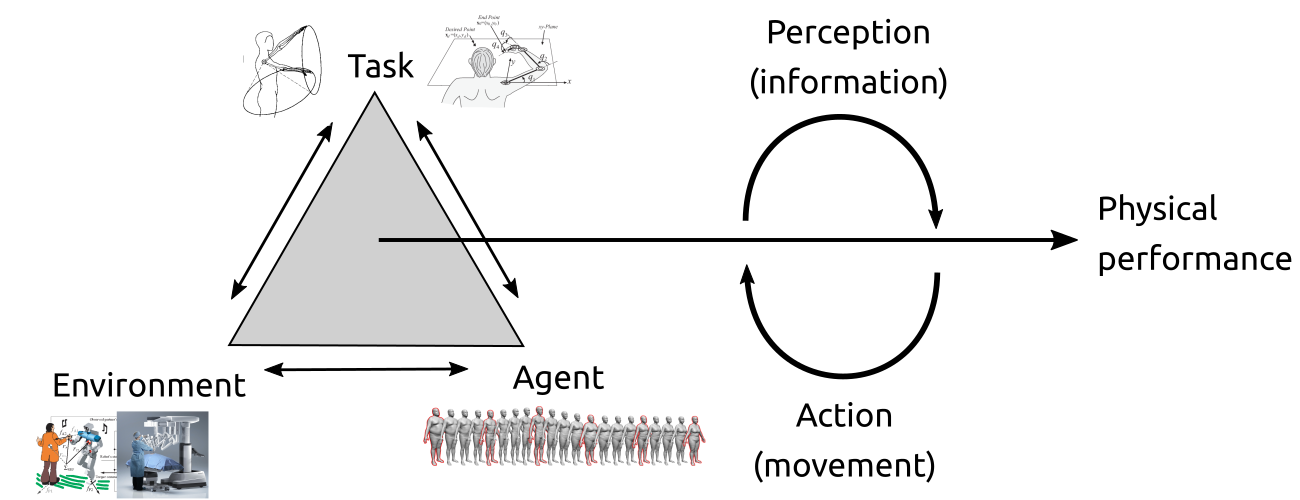
\includegraphics[width=1.0\linewidth]{./figs/modeling-movement/versions/drawing-v00.png}
	%\caption{Newell's model of movement constrains} 
   \end{figure}
\end{frame}
}



%%%%%%%%%%%%%%%%%%%%%%%%%%%%%%%%%%%%%%%%%%%%%%%%%%%%%%%%
{
\paper{
Stergiou et al. 2006 in {\bf Neurologic Physical Therapy};
Stergiou and Decker 2011 in {\bf Human Movement Science};
Tononi et al. 1998 in {\bf Trends in Cognitive Sciences}
}
\begin{frame}{Modelling Movement Variability}
    \begin{figure}
        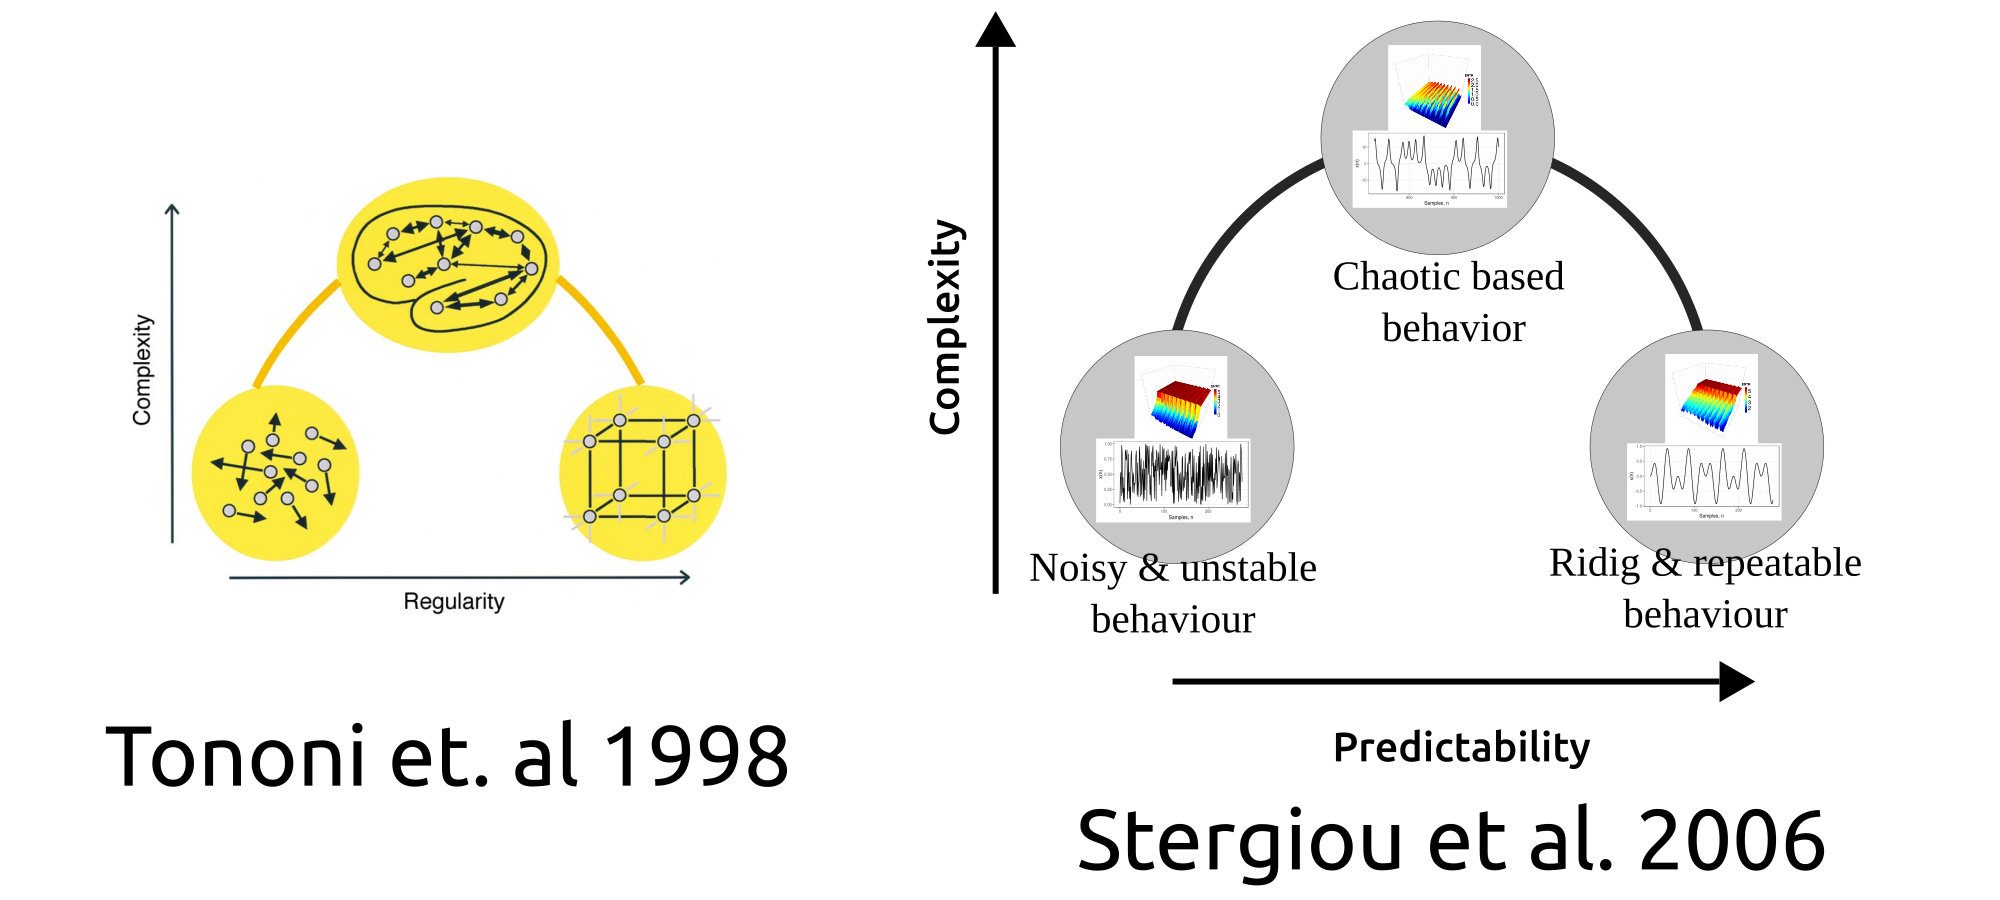
\includegraphics[width=0.95\linewidth]{./figs/modeling-movement-variability/versions/drawing-v00.png}
	%\caption{Theoretical Model of Optimal Movement Variability}
   \end{figure}
\end{frame}
}

